% chain-intersection.tex

\documentclass{standalone}
\usepackage{tikz}
\usetikzlibrary{positioning}

\begin{document}
\begin{tikzpicture}[node distance = 0.00cm]
  \node (abcd) [] {
\includegraphics[scale = 0.20]{chain-abcd}};
  \node (cap1) [right = of abcd] {$\cap$};
  \node (acbd) [right = of cap1] {
\includegraphics[scale = 0.20]{chain-acbd}};
  \node (cap2) [right = of acbd] {$\cap$};
  \node (acdb) [right = of cap2] {
\includegraphics[scale = 0.20]{chain-acdb}};

  \node (eq) [right = of acdb] {$=$};
  \node (poset-abcd-hasse-1) [right = of eq] {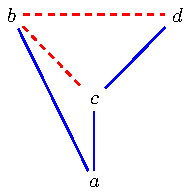
\includegraphics[scale = 0.20]{poset-abcd-hasse-1}};
\end{tikzpicture}
\end{document}

